\chapter{Introduction}
\label{chapter:intro}

% Motivation
There is a great need of robotic pick-and-place systems in many domains, ranging from warehouse automation, service robots, or grocery stores.
Recently more and more robots applied to works in the factory assembly production line or warehouse to reduce human labors. The world-class competitions of Amazon Picking/Robotics Challenges (APC/ARC) 2015-2017 further brought together the teams to develop the picking systems for known or unknown objects from the shelves or totes. The common workflow for picking tasks, especially the solutions for APC/ARC, involve the localization of individual objects via pixel-wise semantic segmentation (e.g. Fully Convolution Networks~\cite{long2015fully}) or bounding-box-based object detection (e.g. Faster RCNN~\cite{ren2015faster}, SSD~\cite{liu2016ssd}, YOLO~\cite{redmon2016you}, etc), estimation of object poses (e.g., geometric model fitting methods such as iterative closest points~\cite{pomerleau2013comparing}), selection of objects to pick (e.g, estimate the probability of picking success~\cite{zeng2018robotic}), and grasping the selected objects. Predicting grasping locations using learning approaches have also been extensively studied~\cite{redmon2015real, mahler2016dex1, mahler2017dex, mahler2017dex3}.

\begin{figure}[t]
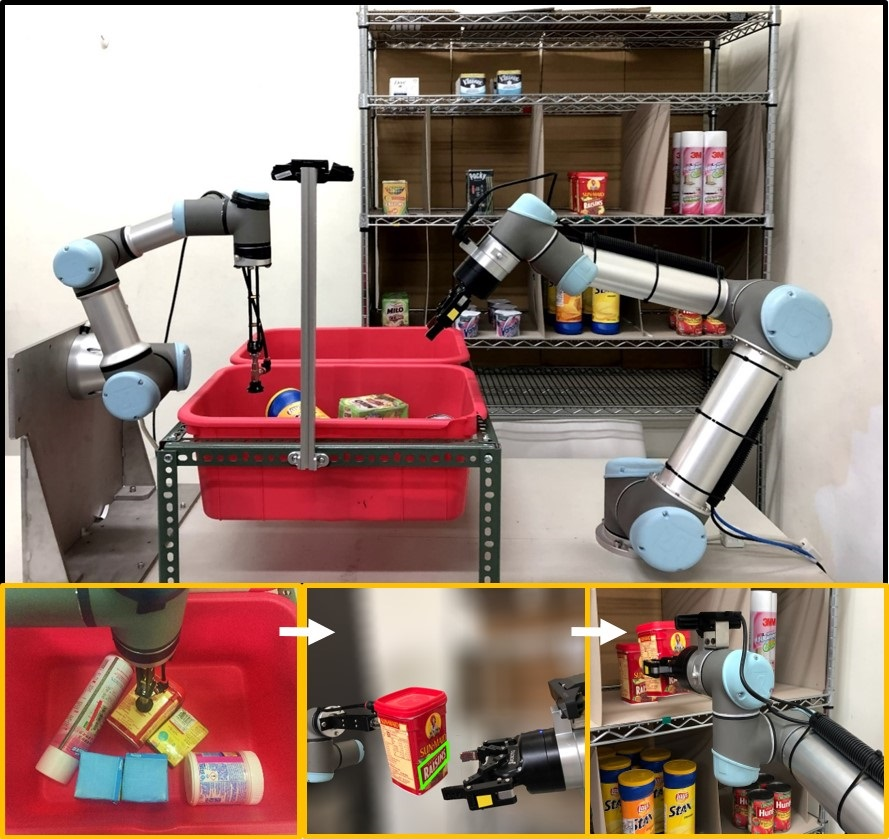
\includegraphics[width=1.0\columnwidth]{./figures/pose-aware-placing-teaser-v3.jpg}
\centering
\caption{We utilize product brandname, one of the ``semantic labels,'' for pose-aware placing. We carry out active manipulation with two cooperative robotic arms to handle object occlusions (e.g., brandname facing down). Bottom left to right: a vacuum gripper picks a target object using object-level or brandname-level affordance prediction, the brandname is then used to predict grasp, and finally a two-finger gripper complete placing.}
\end{figure}

% The importance of pose-aware placing

Although picking and grasping prediction have been addressed, \emph{placing} is still not much addressed in previous work, especially when an object needs to be placed not just by its geometry. Such scenarios include product stocking, inventory taking, checkout, and others. When human customers do the shopping in a store or supermarket, they intuitively pay attention to brandname printed on the product, and therefore the products have to be placed on the shelves with the brandname facing outward. It is usually needed for a human cashier to find where the barcode is printed to identify each product while customers checkout. Therefore, estimates of semantics and geometry of object for pose-aware placing are important to create practical values.

\begin{figure*}[htb]
   \centering
     \begin{subfigure}[t] {0.43\textwidth}
          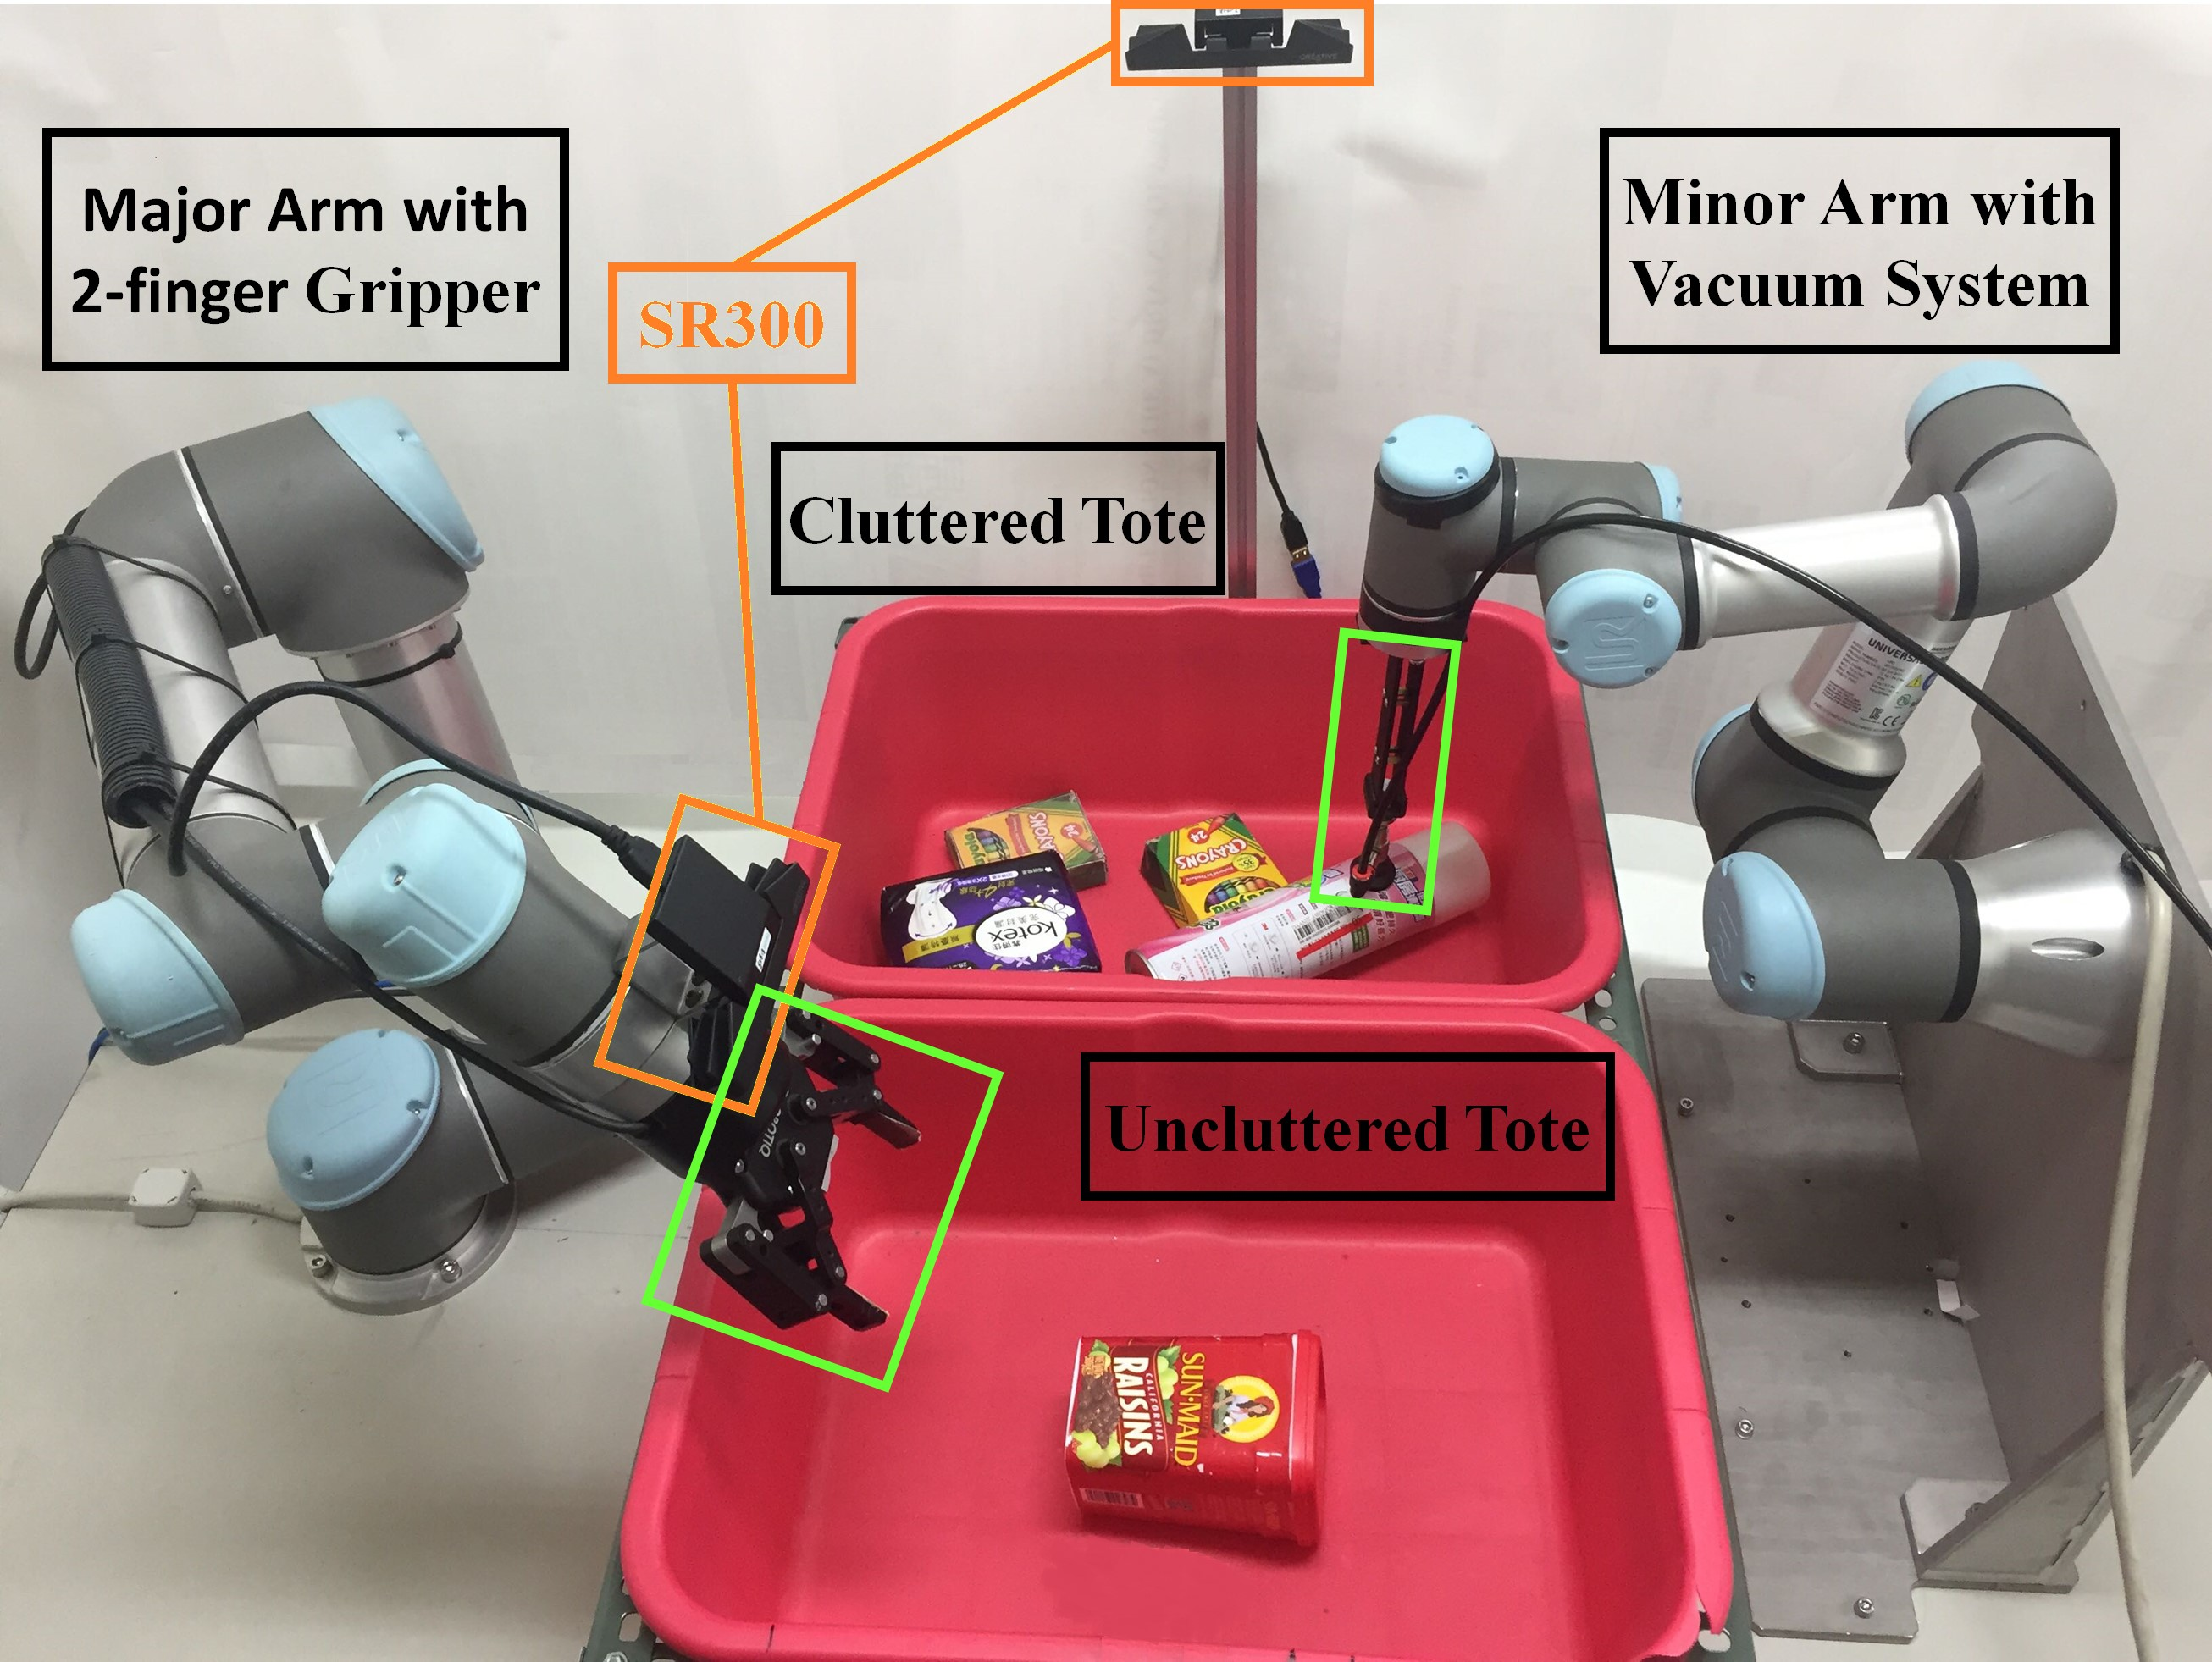
\includegraphics[width=\textwidth]{./figures/robot_system_v2.jpg}
          \caption{Collaborative robotic arms for pose-aware placing. }
 	\label{fig:robot_system}
      \end{subfigure}
     \begin{subfigure}[t] {0.53\textwidth}
          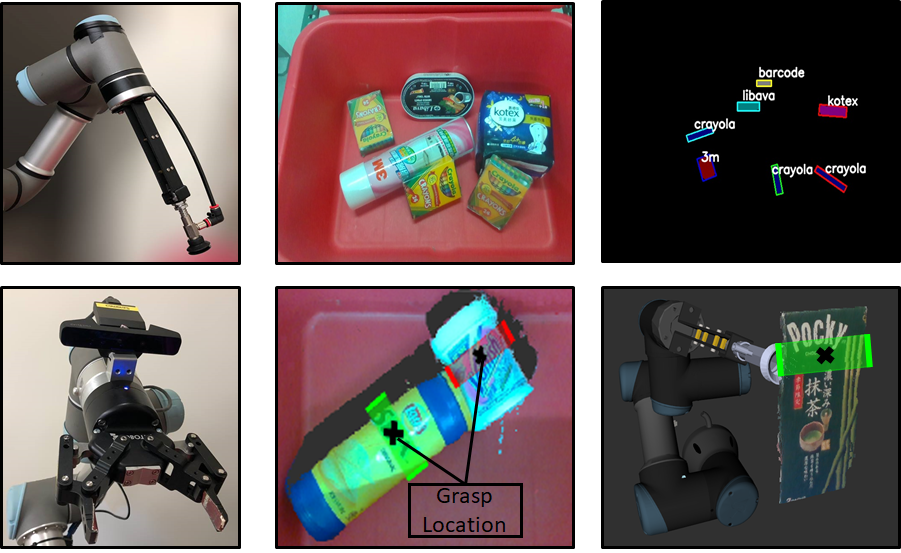
\includegraphics[width=\textwidth]{./figures/affordance_v3.png}
          \caption{Brandname-based affordance and grasp predictions. }
	\label{fig:brandname-direction}
      \end{subfigure}
   \caption{Left: we propose a dual-arm cooperative system to \emph{actively} manipulate the scene to improve perception for placing. The gripper arm moves an occluding object to reveal information (the invisible brandname) hidden underneath, and the two-finger arm further predicts grasp using the brandname and completes pose-aware placing. Right: brandname can be used to predict both affordance for vacuum gripper and grasp for two-finger gripper.
}
\label{fig:baseline-active}
\end{figure*}




% semantic labels: the importance of brandname
We refer a \emph{semantic label} as a piece of surface on an object that provide not just geometry, but also additional information to facilitate manipulations, such as a reference of a task-relevant object pose, better object duplicates handling, or inferring how to perform proper sequence of actions. There may be more than one semantic labels on an object, namely brandname, barcode, one of the six faces of a cubic object, soda can lid, and etc. This work focuses on placing task with brandname semantic labels.

This paper presents an end-to-end pose-aware placing system that utilizes brandname as the reference of object pose and affordance of grippers. We contribute as follows:

\paragraph{Brandname-based Affordance Prediction} Brandname is one of the semantic labels on an object, and exists on almost on every commercial product. Brandname is printed on flat surfaces on box containers or curved surfaces on cylinders, and bounded by a rectangle box. With such property, we can utilize the visibility of brandname to directly predict object affordance (the probability of picking success) for vacuum gripper or grasp for two-finger gripper.

\paragraph{Active Manipulation with Actions of Two Cooperative Arms and Grippers} Other than \emph{passively} using the result of object detection and pose estimation, we present schemes to \emph{actively} manipulate the captured images in order to maximize the visibility of brandnames and individual objects. Our schemes can not only change the camera viewpoint to see the brandname with least occlusion, but also cooperate multiple robotic arms and grippers to manipulate the object, in order to achieve the desired placing.

\paragraph{A Benchmark Dataset with Semantic Labels} Despite the recent progress of object segmentation, training a deep convolution neural network usually requires a huge dataset of labeled training data. Although there has been attempts to handle the constraints of novel objects and limited data, the progress is still limited. In order to train the vision algorithms for semantic labels (brandname and barcode), we construct a dataset that include over 8,000 manually-labeled images with brandnames. The dataset consist of 20 objects, and each with brandname and barcode labels. The dataset includes training data of real and virtual environments, a physical benchmark test set for carrying out placing tasks. The datasets are made publicly available~\cite{textpnp}.


The remainder of the paper is organized as below. Section~\ref{sec:related} describes the related work on recent advances of affordance prediction, as well as active vision and manipulation. We will describe the proposed cooperative dual-arm system in Section~\ref{sec:system}, and how baseline and active manipulation are performed in Section~\ref{sec:active}.  Section~\ref{sec:dataset} describes the ``Brandname Benchmark Dataset'' including training data from real and virtual environments, and a testing set with clutter for evaluations. Section~\ref{sec:exp} provide extensive experiments for the proposed methods on the datasets. Finally, we discuss the future work in Section~\ref{sec:conclusions}.
